\chapter{Emerging Wireless Networks}
We now further our system overview into some new, emerging systems.

\section{Ad-hoc Networks}
Ad-hoc wireless networks are an emerging wireless system, initially 
developed for military purposes. \mKeyword{Ad-hoc networks} are networks without
a fixed infrastructure, where you don't have an access point, nor a backbone 
infrastructure to your network. The network is made up of equal nodes and based 
on peer-to-peer communications. To reach nodes that are too far away from the 
sender, we exploit multihopping. We could memorizing the network's routing 
scheme, but note that we have a dynamic network topology! So, since you don't 
usually know where you're going, you can't use the more common routing 
protocols. 

\begin{figure}[t]
  \centering
  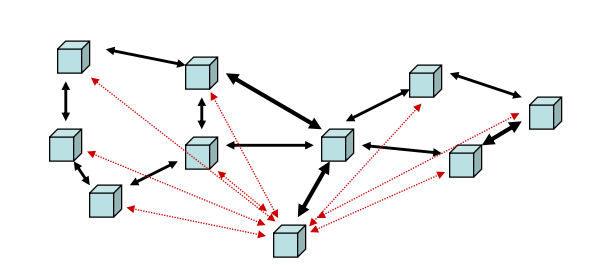
\includegraphics[width=0.8\linewidth]{AHNetwork.png}
  \caption{Ad-Hoc Network}				
  \label{fig:ewn:AHNetwork}
\end{figure}

Ad-hoc Networks are very flexible, useful for many emerging 
applications. The capacity of such networks is generally unknown because 
depending on which node is transmitting, the nearby nodes will be blocked to 
avoid interference. 
Consider this structure (capital letters are nodes, arrows represent 
links):
\begin{equation*}
B \leftrightarrow A \leftrightarrow C \leftrightarrow D
\end{equation*}

If D wishes to transmit to C while A transmits to B, it wouldn't be able 
to do it because C is already occupied with A's messages (interference!).
Furthermore, we never really know the size and routing of our network, 
both can change very frequently.
In this kind of networks \textbf{\mKeyword{crosslayer design}} is critical
for efficiency and very challenging.
Finally, energy constraint impose interesting design tradeoffs for 
communication and networking: for example, choosing to increase transmission 
power to avoid multihop leads to problems both in energy consumption (remember, 
if the distance doubles, the energy required is four time greater) and
interference. I may occupy the whole network for just one transmission. 

\subsection{Sensor Networks}
Sensor Networks are a specific type of ad-hoc networks. You have 
different sensors, each used to monitor a specific thing. The driving constraint 
is energy, since sensors usually have a limited amount of energy and are powered 
by non-rechargeable batteries. To spare energy, they are usually turned off and 
periodically turn on to monitor the environment. 	When they are on, they 
may help other sensors to send messages, even if a very good synchronization is
needed. 
Usually these networks are very large (up to 100,000 nodes) but, unless 
they are sending pictures of the environment, nodes have a low per-node rate, 
sending very simple data: temperature values, pollution levels, water 
levels\dots
The data flows to a centralized location that then analyzes, processes 
or sends it farther away.
It is important not to lose packets, so aggregating should be mitigated 
to avoid losing big portions of data. Also, avoid big delays, since data is 
highly correlated in time and space.

\subsubsection{Underwater Sensor Networks}
Main challenge: electromagnetic waves don't propagate well in water, so 
one has to resolve other forms of communication, for example sound waves.
Using sound waves means that the connection will be much slower (sound 
speed instead of light speed). On the other hand, two waves transiting at the
same time but far enough from each other will not collide. Remember: there is a 
collision if the receiver receives at the same time two different signals, not 
when two messages travel together.
As for battery consumption, they usually rely on battery.

\subsection{Mobile Ad-Hoc Networks (MANET)}
These are ad-hoc networks with a focus on mobility. They were initially 
used for military purposes and then extended to civilian tasks. The topology of 
the network continuously changes and the protocol used has to adapt 
consequently, keeping into account that every information received may already 
be obsolete. In some cases, one may need to resolve to flooding. Like ad-hoc 
networks, they are deployable, re-configurable and portable. They may be created 
to satisfy a temporary need.

\subsubsection{Vehicular ad-hoc Networks (VANET)}	

\begin{figure}[t]
  \centering
  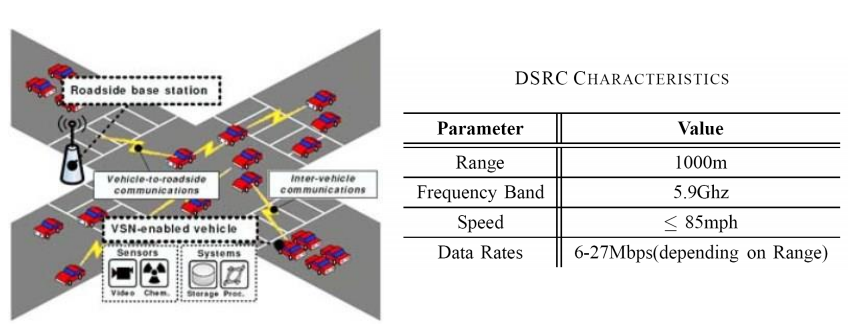
\includegraphics[scale=0.49]{VANET}
  \caption{Vehicular ad-hoc Networks (VANET)}
  \label{fig:mn:VANET}
\end{figure}

Note that, when considering vehicles, since they have an engine, 
reducing energy consumption isn't a priority. Even further, a group of vehicles 
on a road moving in the same direction move together in respect to each-other. 
The technology for automated vehicles is already present, the two main concerns 
are:
\begin{enumerate}
\item Legal problems: in case of accidents, whose fault is it?
\item Moral decisions: if a car has to steer to avoid an 
  accident but in doing so it hits a passer-by, what is the best decision?
\end{enumerate}
Accidents are estimated to occur mainly when having automated cars mixed 
with regular cars (SW malfunctioning or hijack may still occur but are the 
secondary concern now). In a controlled environment we can monitor, while people 
are unpredictable. 
Finally, there is already a frequency reserved for vehicles 
communication (Standard IEEE 802,11p).

\subsection{Opportunistic ad-hoc Networks}
Opportunistic Nets were driven by commercial application needs and 
designed for when there may be an available Internet connection, but we try to 
replace it opportunistically with an ad-hoc network. Basically, they don't use 
homogeneous nodes (like in traditional ad-hoc) but, instead, always try to use 
the best available. Their main feature is flexibility.

\section{Mesh Networks}
Mesh Networks are something between ad-hoc networks and wireless ones. 
They are different because the can connect to both regular and completely 
wireless access points. In this sense, they are ad-hoc opportunistic extensions 
of a fixed urban infrastructure.
Their main purpose is to create a low-cost, easily deployable, high 
performance wireless coverage. When designing a Mesh Network, one must carefully 
choose the routing protocol, considering all the types of connection you may 
need. Routing protocols have to achieve fairness and local balancing, also 
remembering that in multihop, having two nodes communicate may prevent others in 
range.
Finally, it is difficult to determine a quality of service, that is 
stating a quality standard and being able to assure it.

\begin{figure}[!h]
  \centering
  %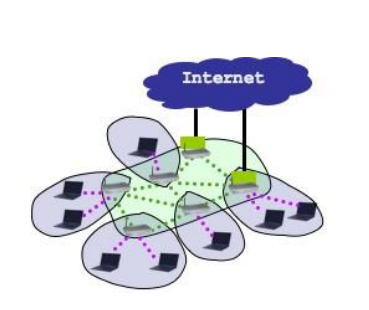
\includegraphics[width=0.8\linewidth]{MeshNetwork.png}
  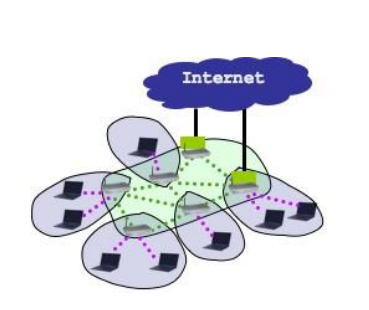
\includegraphics[scale=0.6]{MeshNetwork}
  \caption[An example of a Mesh Network]{Mesh Network (the green ones are
   regular access points)}
  \label{fig:mn:MeshNetwork}
\end{figure}	

\section{Distributed Control over Wireless Links}
These networks deal with automated vehicles: cars, Unmanned Airborne 
Vehicles (UAV), insect fliers and so on.
In these kind of networks it is important to have a good control of the 
environment, so it is important to avoid packet loss and/or delays and also 
assuring a good bandwidth and speed when delivering messages. Avoid queues since 
they cause delays.
The controller design should be especially robust to network faults.

\section{Radio Frequency Identification (RFID)}
RFIDS are based on magnetic fields and are usually tags without a 
battery (even though they can have it). They store more info than a simple 
barcode and are therefore used in supply chains instead of them. They don't 
need a direct optical reading but, instead, require an emitter of 
electro-magnetic waves that charge the tag. The charged tag sends a message 
containing all the information back to the server, that can then check it.
Even though it contains more information that a simple barcode, it is 
more expensive. Their popularity is increasing, and standards are currently 
under development.

\begin{figure}[t]
  \centering
  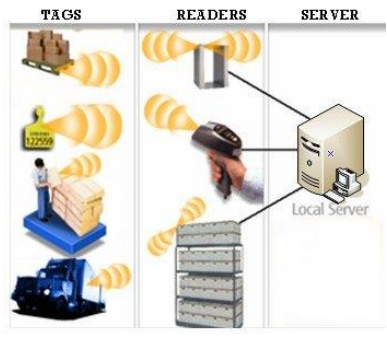
\includegraphics[scale=0.6]{RFID}
  \caption{Radio Frequency Identification (RFID)}
  \label{fig:ewn:RFID}
\end{figure}

\section{Nano-Networks}
Networks made up of very tiny objects and very small distances. You 
can't just replicate in scale what you would normally do  but instead you have 
to rely on different means of communication, very popular are calcium signals.

\begin{figure}[t]
  \centering
  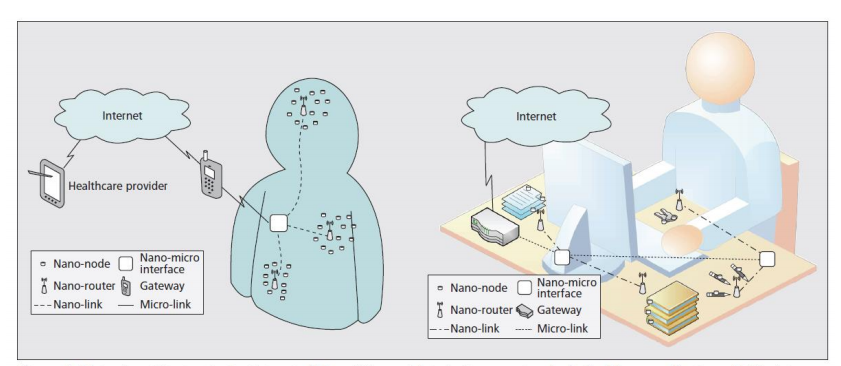
\includegraphics[scale=0.5]{NanoNet}
  \caption{An example of nano-network}				
  \label{fig:ewn:NanoNet}
\end{figure}


